%\documentclass[10pt,fleqn]{article} % Default font size and left-justified equations
%\usepackage[%
%    pdftitle={Modélisation SLCI : Stabilité des systèmes},
%    pdfauthor={Xavier Pessoles}]{hyperref}
%    
%\input{style/new_style}
%\input{style/macros_SII}
%\usepackage{multicol}
%\usepackage{siunitx}
%\fichetrue
%%\fichefalse
%
%\proftr

%%%% Paramétrage du TD %%%%
\def\xxactivite{Application}
\def\xxauteur{\textsl{Xavier Pessoles}}


\def\xxnumchapitre{Chapitre 1 \vspace{.2cm}}
\def\xxchapitre{\hspace{.12cm} Stabilité des systèmes}

\def\xxcompetences{%
\textsl{%
\textbf{Savoirs et compétences :}\\
\vspace{-.4cm}
\begin{itemize}[label=\ding{112},font=\color{bleuxp}] 
%\item \textit{Mod3.C2 : } pôles dominants et réduction de l’ordre du modèle : principe, justification
%\item \textit{Res2.C4 : } stabilité des SLCI : définition entrée bornée -- sortie bornée (EB -- SB)	
%\item \textit{Res2.C5 : } stabilité des SLCI : équation caractéristique	
\item \textit{Res2.C6 : } stabilité des SLCI : position des pôles dans le plan complexe
\item \textit{Res2.C7 : } stabilité des SLCI : marges de stabilité (de gain et de phase)
\end{itemize}
}}


\def\xxfigures{
%\includegraphics[width=3cm]{SoloWheel_Orbit}\\
%\textit{}
}%figues de la page de garde

\def\xxtitreexo{Application}
\def\xxsourceexo{\hspace{.2cm} \footnotesize{Xavier Pessoles}}


\def\xxactivite{Application \ifprof  -- Corrigé \else \fi}
%\def\xxauteur{\textsl{P. Dupas.}}


\iflivret
\input{\repRel/Style/pagegarde_TD}
\else
\input{\repRel/Style/pagegarde_TD}
\fi
\setlength{\columnseprule}{.1pt}

\pagestyle{fancy}
\thispagestyle{plain}


\vspace{4.5cm}

\def\columnseprulecolor{\color{bleuxp}}
\setlength{\columnseprule}{0.4pt} 

%%%%%%%%%%%%%%%%%%%%%%%





\ifprof
\else
\begin{multicols}{2}
\fi

%\subsection*{Exercice 1 -- Réponse impulsionnelle (entrée Dirac)}
\setcounter{numques}{0}
On considère le schéma-blocs suivant. 
\begin{center}
\includegraphics[width=\linewidth]{fig_01}
\end{center}

On donne ci-dessous la réponse indicielle pour $K_C=1$.

\begin{center}
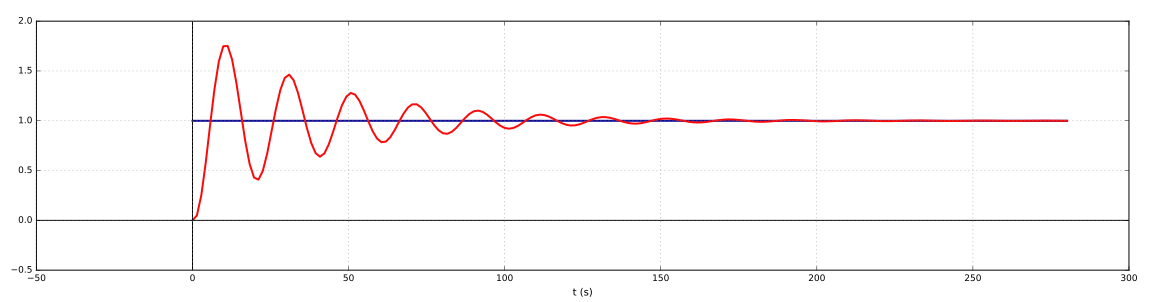
\includegraphics[width=\linewidth]{fig_02}
\end{center}


\question{Justifier l'allure du diagramme du diagramme de Bode donné ci-dessous pour $K_C=1$.}

\question{Donner graphiquement les marges de phase et de gain pour $K_C=1$.}
\ifprof
\begin{center}
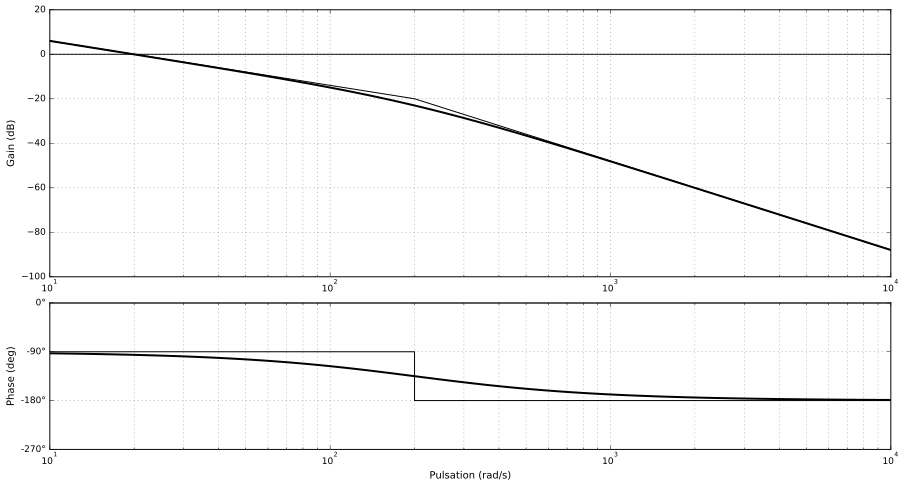
\includegraphics[width=\linewidth]{cor_01}
\end{center}

\else
\fi


\question{Donner analytiquement les marges de phase et de gain pour $K_C=1$ (méthode).}
\ifprof
\begin{corrige}
\textbf{Calcul de la marge de gain}
\begin{itemize}
\item On détermine $\omega_{180}$ tel que $\arg\left(\text{FTBO}(j\omega_{180})\right)=-180\degres$. 

$\arg\left(\text{FTBO}(j\omega)\right) $ $= -\arg\left( j\omega\right)-\arg\left( 1+ 10 j\omega\right)-\arg\left(1+0,5j\omega \right) $ $= - 90 - \arctan \left( 10 \omega \right) - \arctan \left( 0,5 \omega \right)$.

$\arg\left(\text{FTBO}(j\omega_{180})\right)=-180\degres$ 
$\Leftrightarrow - 90 - \arctan \left( 10 \omega \right) - \arctan \left( 0,5 \omega \right) = -180$

\begin{python}
import math as m
from pylab import *
from scipy.optimize import bisect 

def f(x):                                       
    res = m.pi/2 - m.atan(10*x) - m.atan(0.5*x)
    return res

zero1 = bisect(f, .1, 10)
\end{python}
On a $\omega=\SI{0,447}{rad.s^{-1}}$.
%$\Leftrightarrow - \arctan \left( 10 \omega \right) - \arctan \left( 0,5 \omega \right) = -90$
\end{itemize}

\end{corrige}
\else
\fi

\question{Le cahier des charges impose des marges de gain et de phase minimales de \SI{12}{dB} et 40\degres. Déterminer
la plus grande valeur de $K_C$ permettant de vérifier ce cahier des charges}


\ifprof
\else
\end{multicols}
\fi



\ifprof
\else

\begin{center}
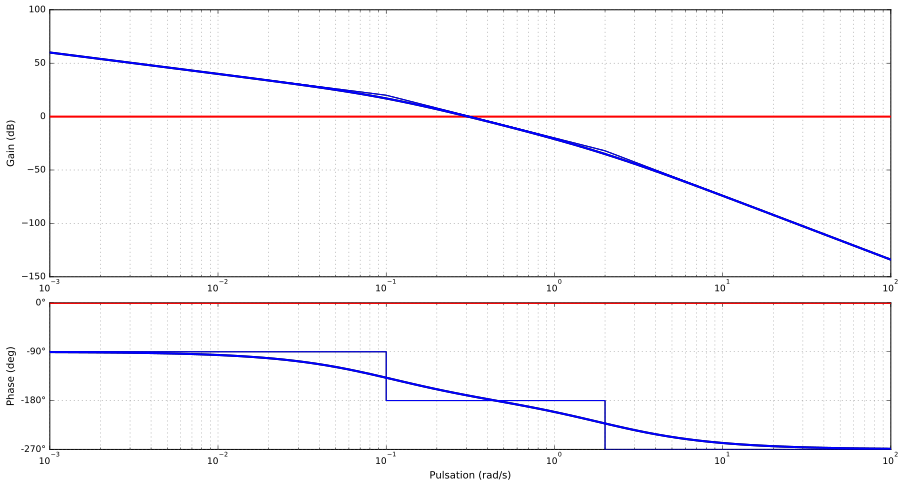
\includegraphics[width=\linewidth]{fig_03}
\end{center}

\fi


\ifprof
\begin{center}
\includegraphics[width=\linewidth]{cor_02}
\end{center}

\else
\fi


%\ifprof
%\else
%\noindent\begin{minipage}[c]{.4\linewidth}
%\begin{center}
%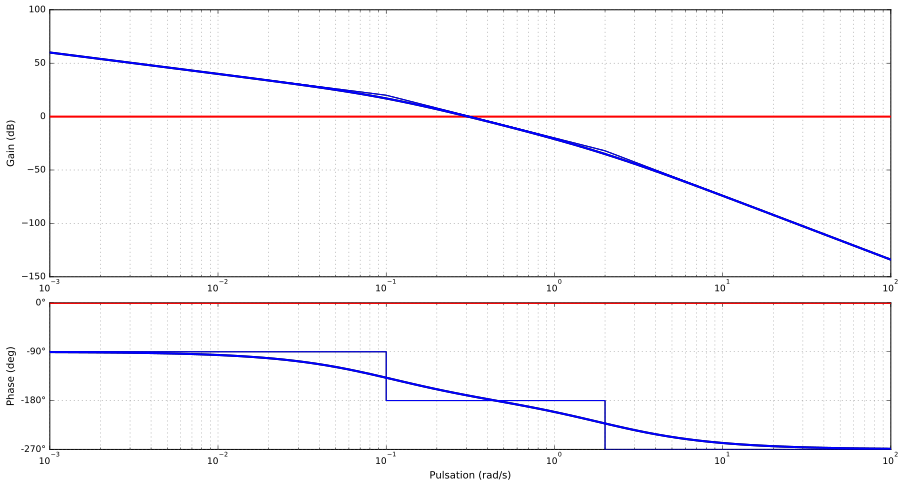
\includegraphics[width=\linewidth]{fig_03}
%\end{center}
%\end{minipage}\hfill
%\begin{minipage}[c]{.46\linewidth}
%\begin{center}
%\includegraphics[width=.9\linewidth]{fig_01}
%\end{center}
%\end{minipage}

\ifprof
\else
\begin{center}
\includegraphics[width=\linewidth]{img_04}
\end{center}
\fi

%
%\begin{center}
%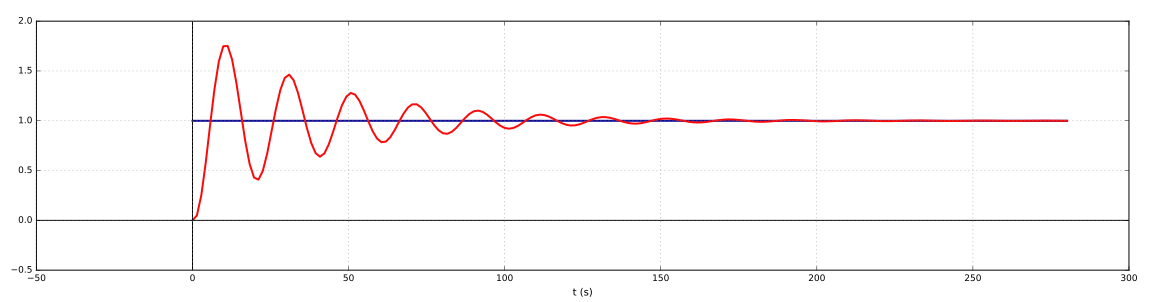
\includegraphics[width=\linewidth]{fig_02}
%\end{center}
%
%\begin{center}
%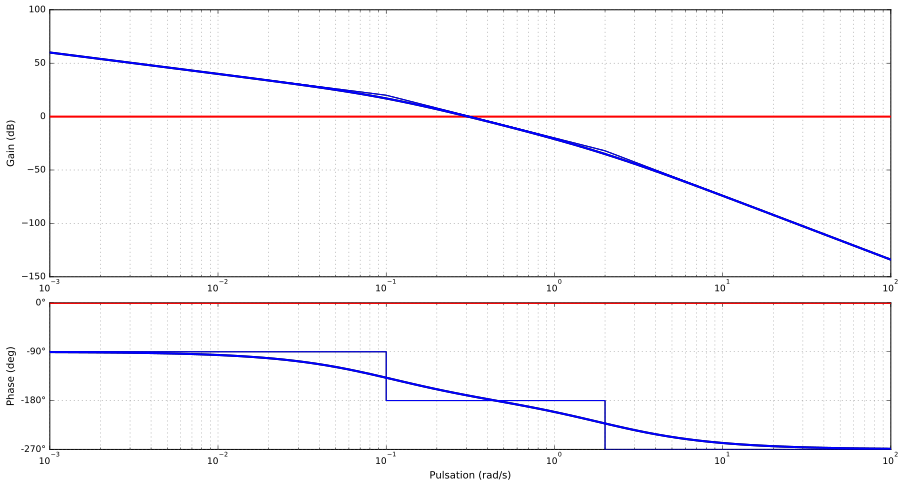
\includegraphics[width=\linewidth]{fig_03}
%\end{center}
%
%\begin{center}
%\includegraphics[width=.8\linewidth]{fig_04}
%\end{center}


%
%\end{document}
%
%\subsection*{Exercice 3 -- Applications du critère du Revers}
%
%\subparagraph*{}\textit{On donne ci-dessous les lieux de transferts de plusieurs FTBO. Déterminer, à l'aide du critère du Revers si les systèmes sont stables en BF.}
%\subparagraph*{}\textit{Pour les systèmes stables déterminer les marges de gain et de phase.}
%
%\end{multicols}
%
%\begin{center}
%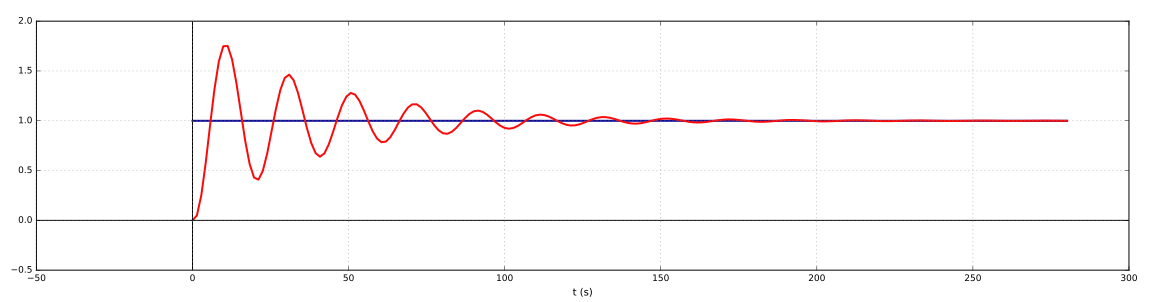
\includegraphics[width=\linewidth]{fig_02}
%\end{center}
%
%\begin{center}
%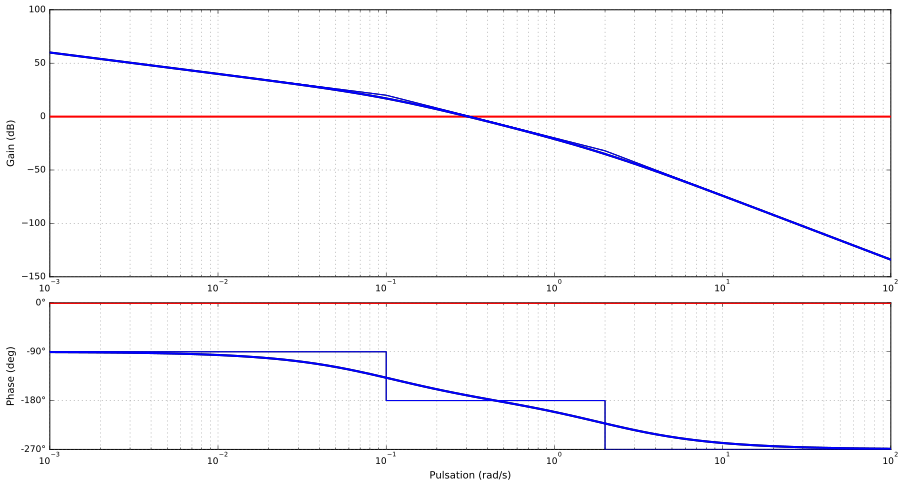
\includegraphics[width=\linewidth]{fig_03}
%\end{center}
%
%\begin{center}
%\includegraphics[width=.8\linewidth]{fig_04}
%\end{center}



